
%% To submit your paper:
%\documentclass[draft,linenumbers]{agujournal}
%\draftfalse

%% For final version.
 \documentclass{agujournal}

\journalname{Global Biochemical Cycles}

\usepackage{bm}
\usepackage{booktabs}
\usepackage{amssymb, amsmath}

\begin{document}


\title{Supplementary material for \\ 
Soil organic matter persistence as a stochastic process: age and transit time distributions of carbon in soils}

\authors{Carlos A. Sierra\affil{1}, Alison Hoyt\affil{1}, Yujie He\affil{2}, Susan E. Trumbore\affil{1}}


% \affiliation{1}{First Affiliation}
% \affiliation{2}{Second Affiliation}
% \affiliation{3}{Third Affiliation}
% \affiliation{4}{Fourth Affiliation}

\affiliation{1}{Max Planck Institute for Biogeochemistry, Hans-Kn\"oll-Str. 10, 07745 Jena, Germany}
\affiliation{2}{Department of Earth System Science, University of California, Irvine, USA}
%(repeat as many times as is necessary)

\correspondingauthor{C.A. Sierra}{csierra@bgc-jena.mpg.de}

%% Keypoints, final entry on title page.

% Example:
% \begin{keypoints}
% \item	List up to three key points (at least one is required)
% \item	Key Points summarize the main points and conclusions of the article
% \item	Each must be 100 characters or less with no special characters or punctuation
% \end{keypoints}

\newpage

%\section{Supplementary Figures}

\begin{figure}[t]
   \centering
   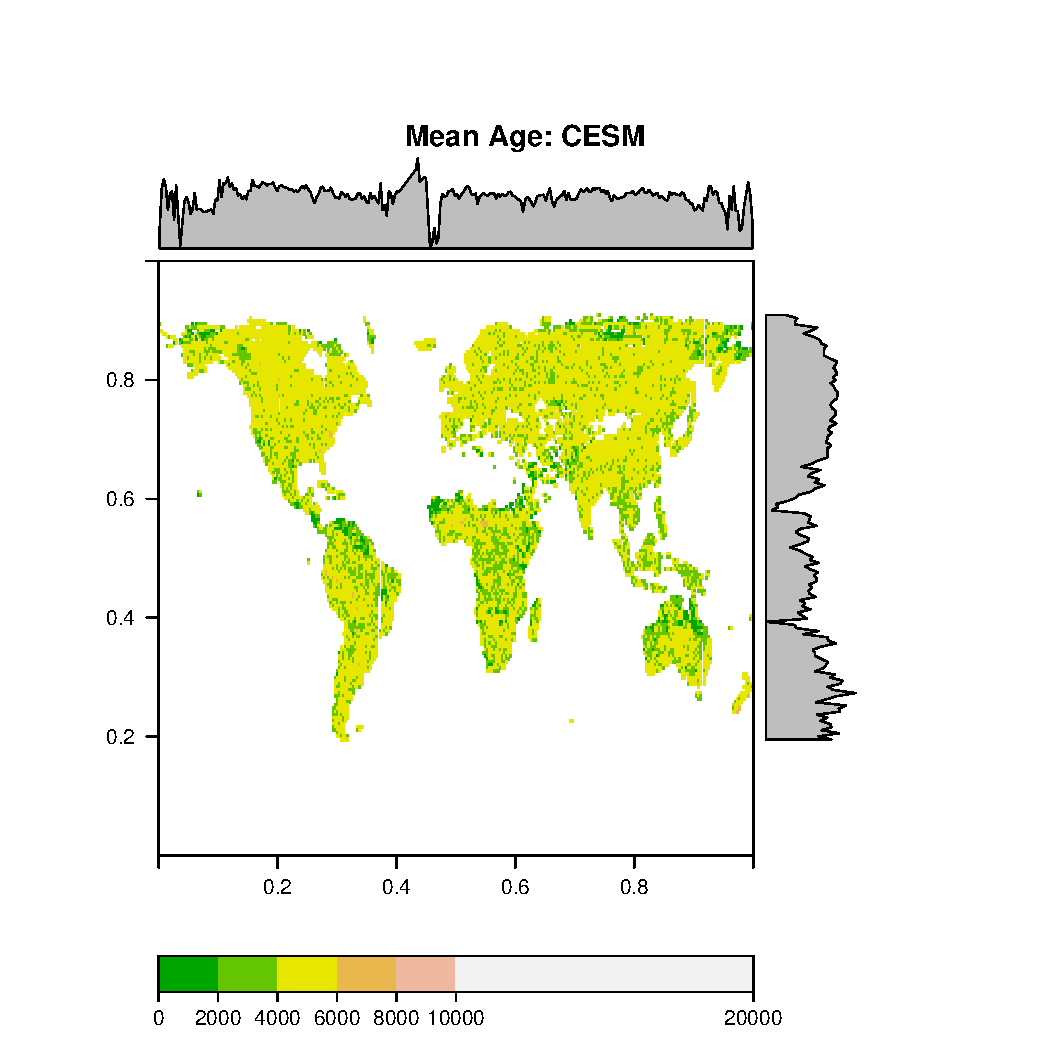
\includegraphics{Figures/mapAcolors_CESM} % requires the graphicx package
   \caption{Mean age of the reduced complexity model CESM calculated for each grid cell. }
\end{figure}

\begin{figure}[t]
   \centering
   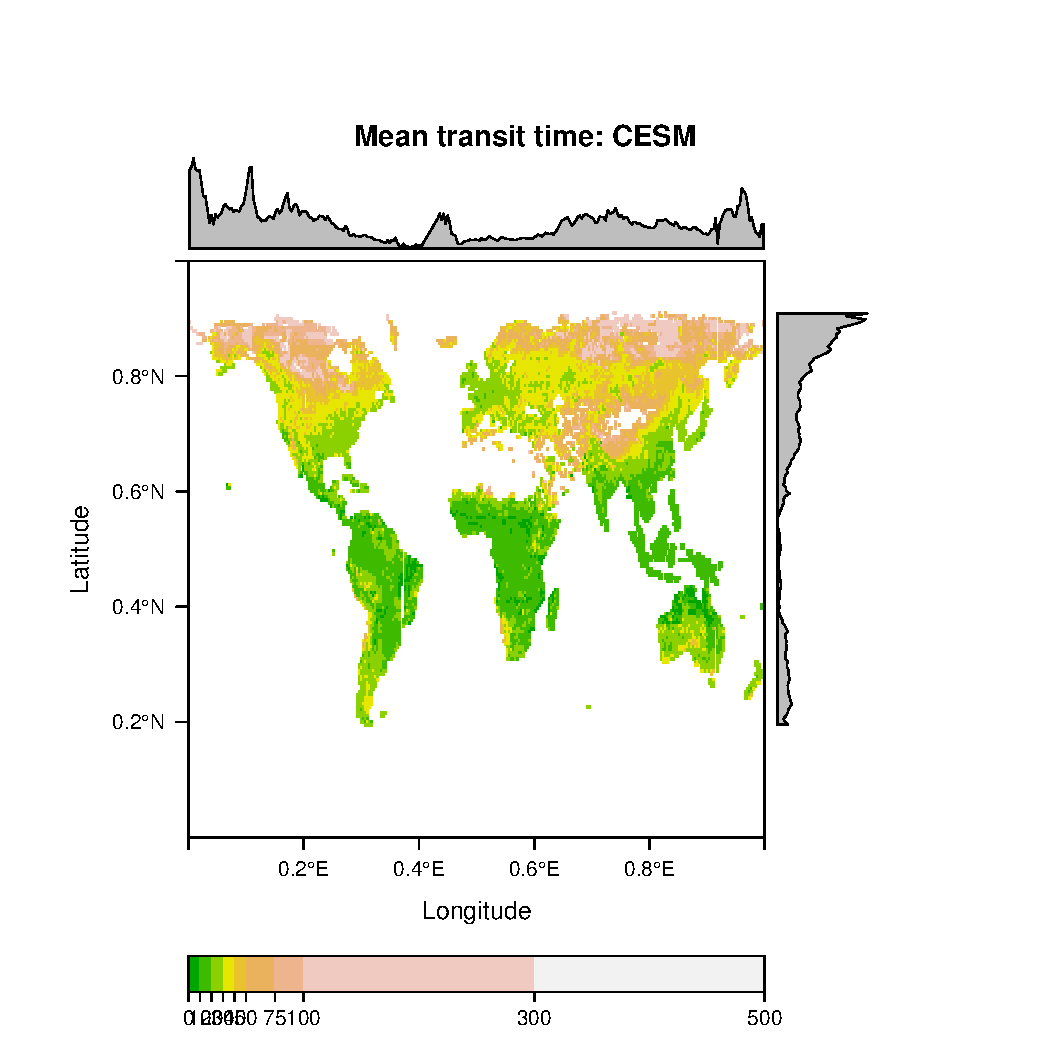
\includegraphics{Figures/mapTTcolors_CESM} % requires the graphicx package
   \caption{Mean transit time of the reduced complexity model CESM calculated for each grid cell. }
\end{figure}

\begin{figure}[t]
   \centering
   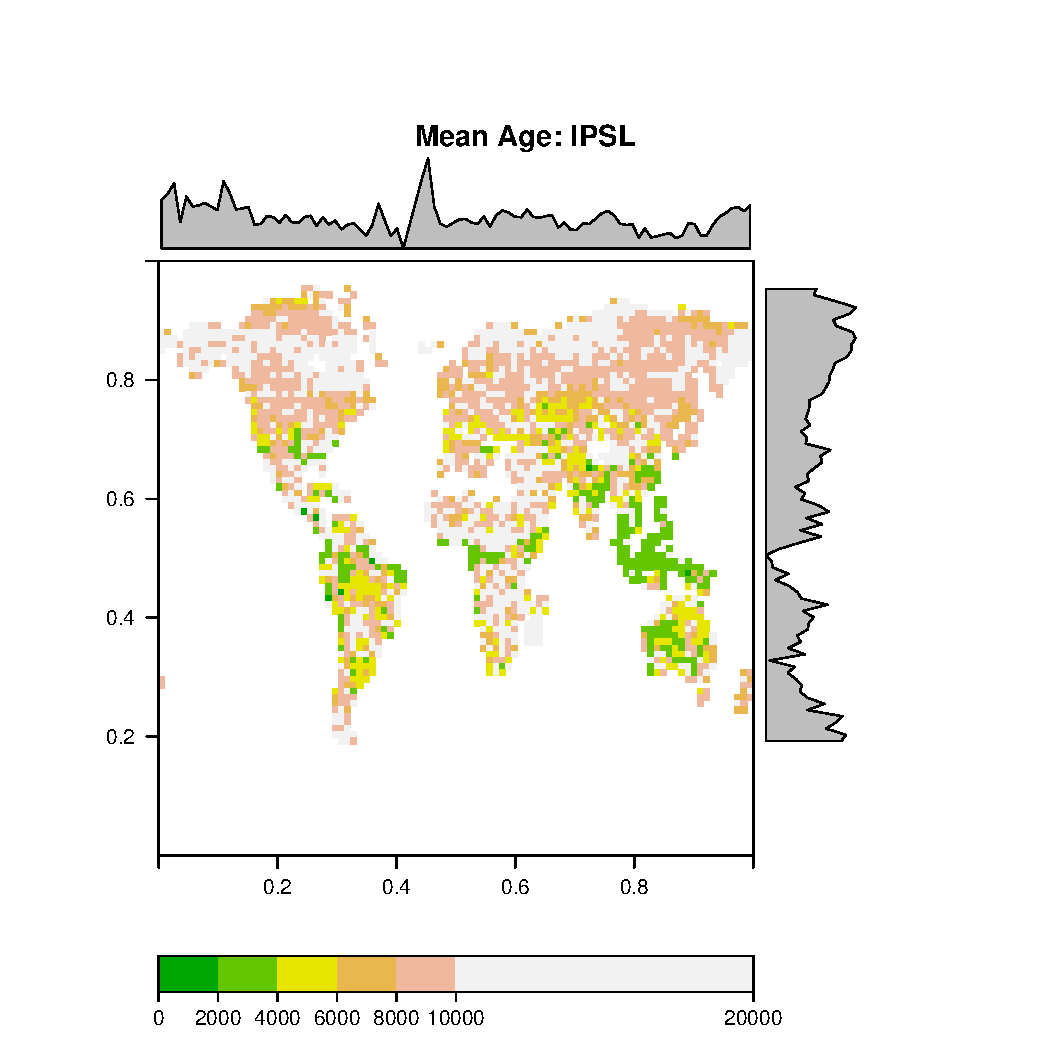
\includegraphics{Figures/mapAcolors_IPSL} % requires the graphicx package
   \caption{Mean age of the reduced complexity model IPSL calculated for each grid cell. }
\end{figure}

\begin{figure}[t]
   \centering
   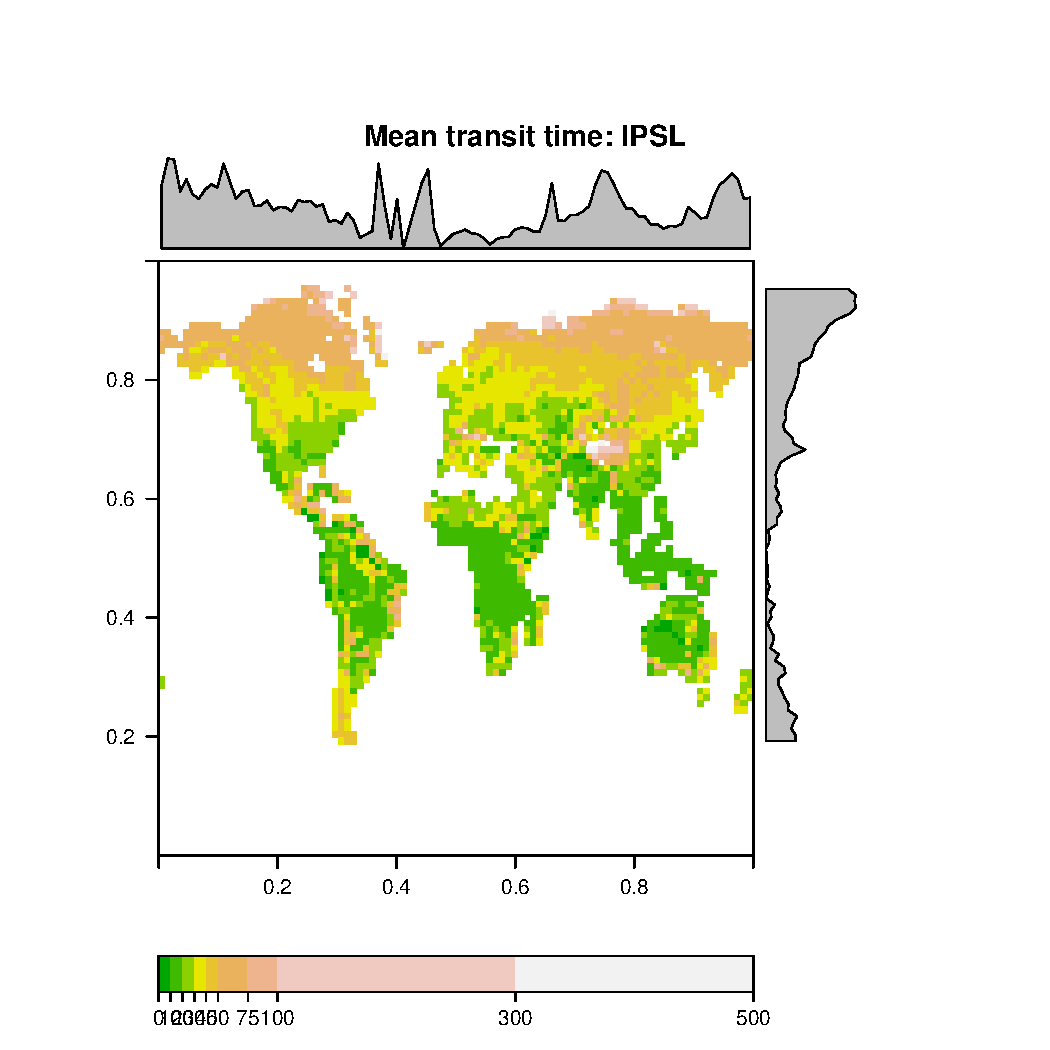
\includegraphics{Figures/mapTTcolors_IPSL} % requires the graphicx package
   \caption{Mean transit time of the reduced complexity model IPSL calculated for each grid cell. }
\end{figure}

\begin{figure}[t]
   \centering
   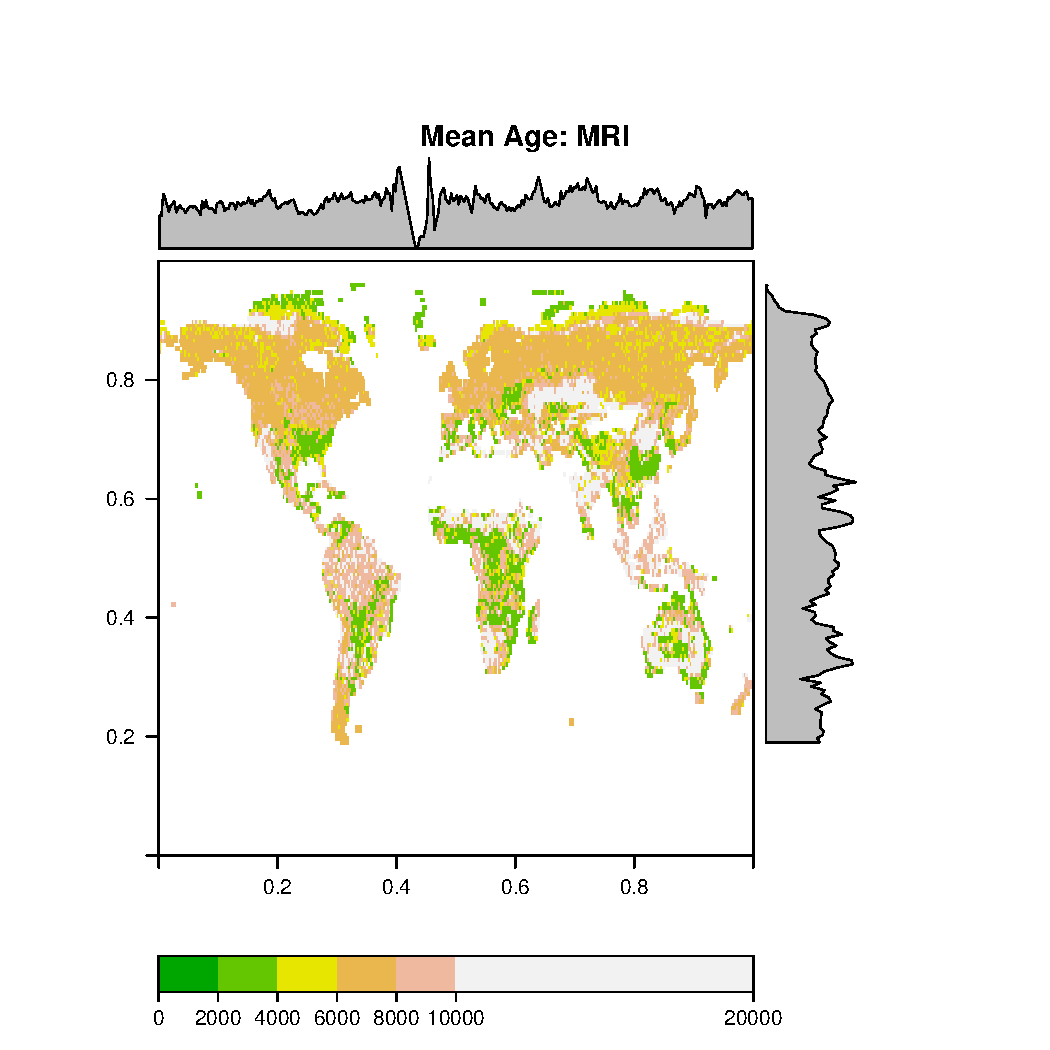
\includegraphics{Figures/mapAcolors_MRI} % requires the graphicx package
   \caption{Mean age of the reduced complexity model MRI calculated for each grid cell. }
\end{figure}

\begin{figure}[t]
   \centering
   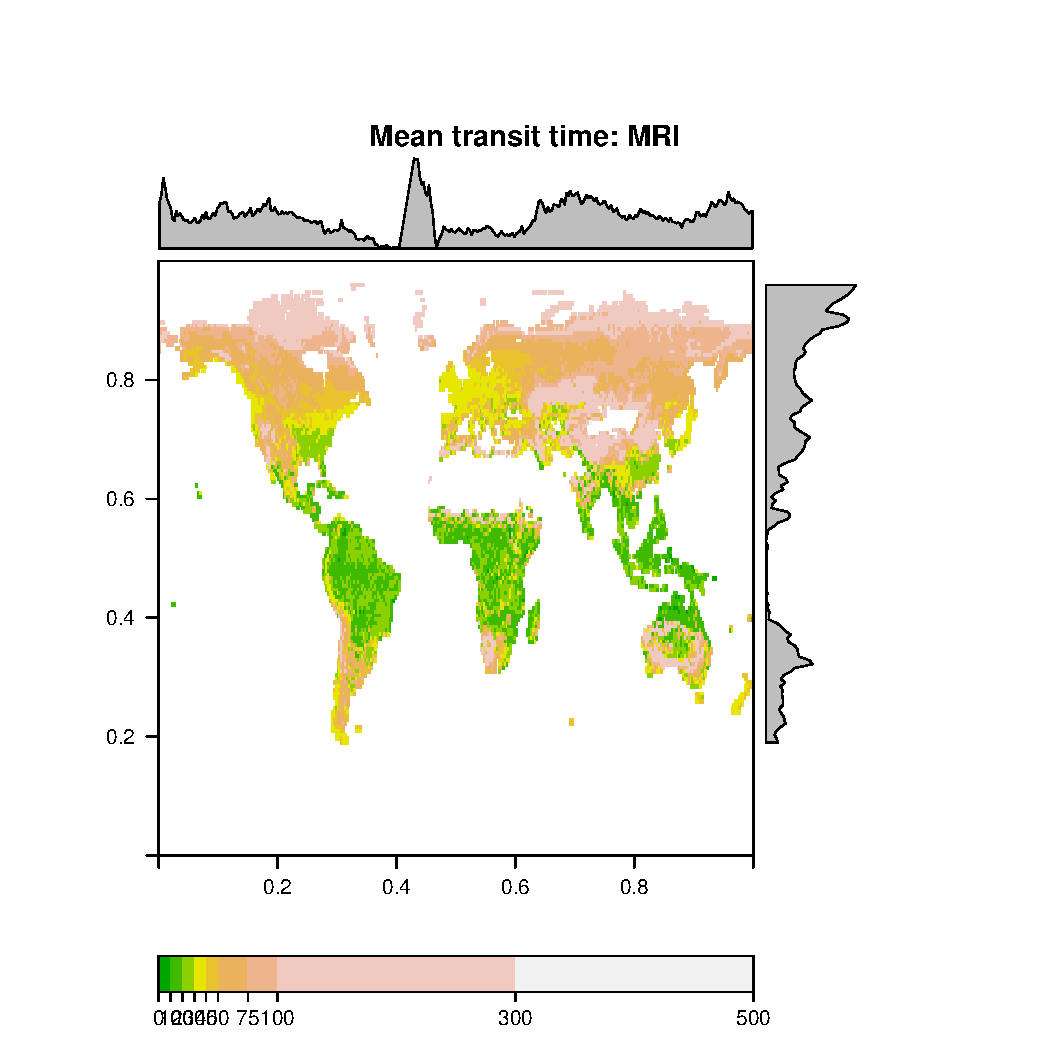
\includegraphics{Figures/mapTTcolors_MRI} % requires the graphicx package
   \caption{Mean transit time of the reduced complexity model MRI calculated for each grid cell. }
\end{figure}

\begin{figure}[t]
   \centering
   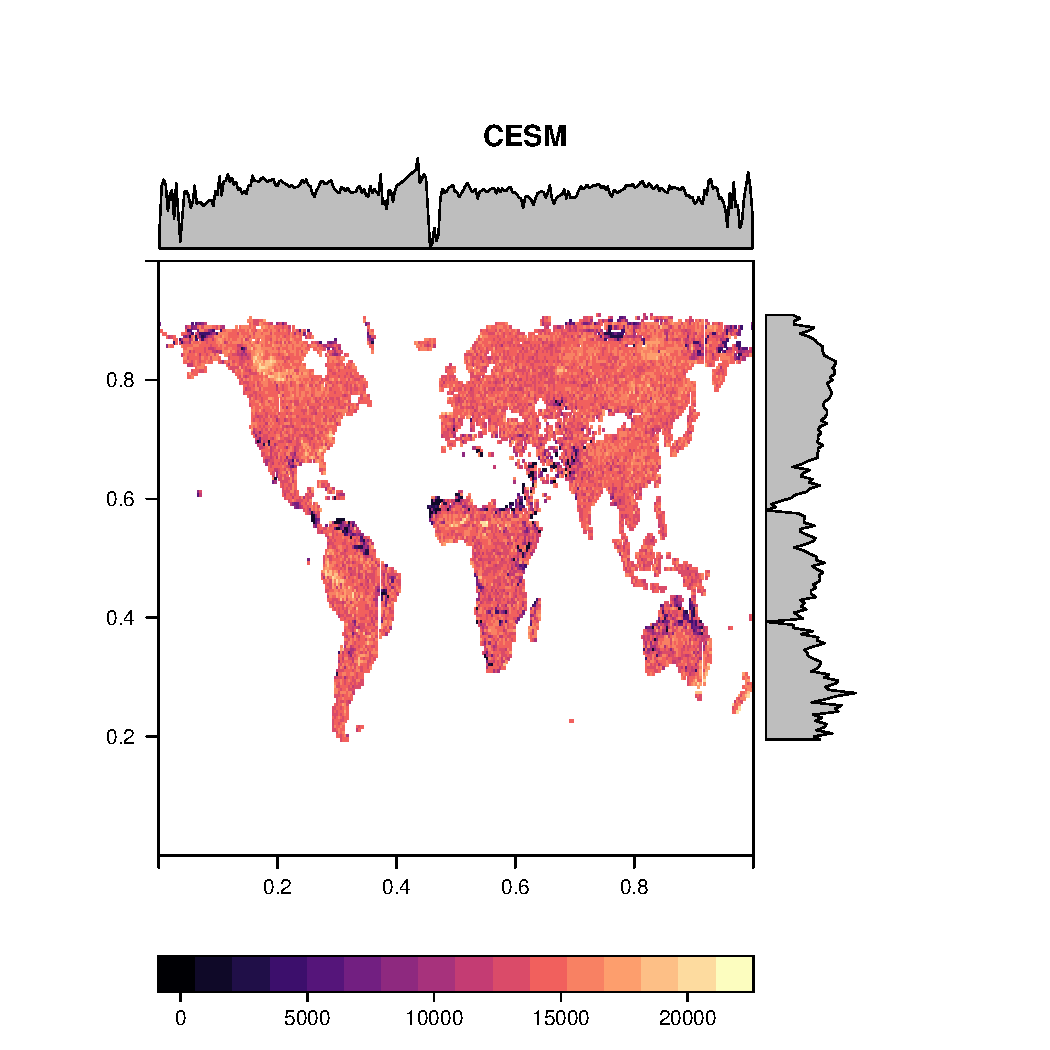
\includegraphics{Figures/corrP95CESM} % requires the graphicx package
   \caption{95\% quantile of the age distribution calculated for the reduced complexity version of the CESM model.}
\end{figure}

\begin{figure}[t]
   \centering
   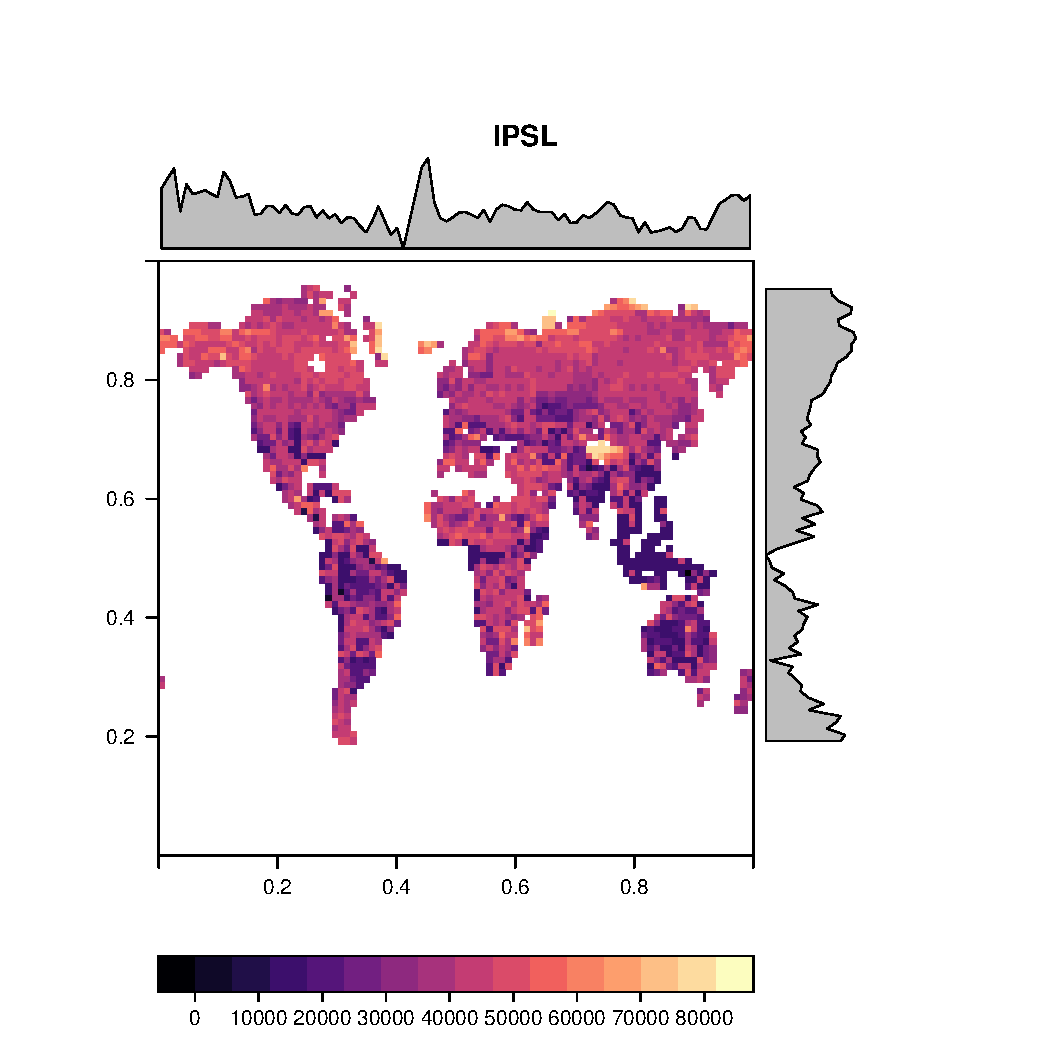
\includegraphics{Figures/corrP95IPSL} % requires the graphicx package
   \caption{95\% quantile of the age distribution calculated for the reduced complexity version of the IPSL model.}
\end{figure}

\begin{figure}[t]
   \centering
   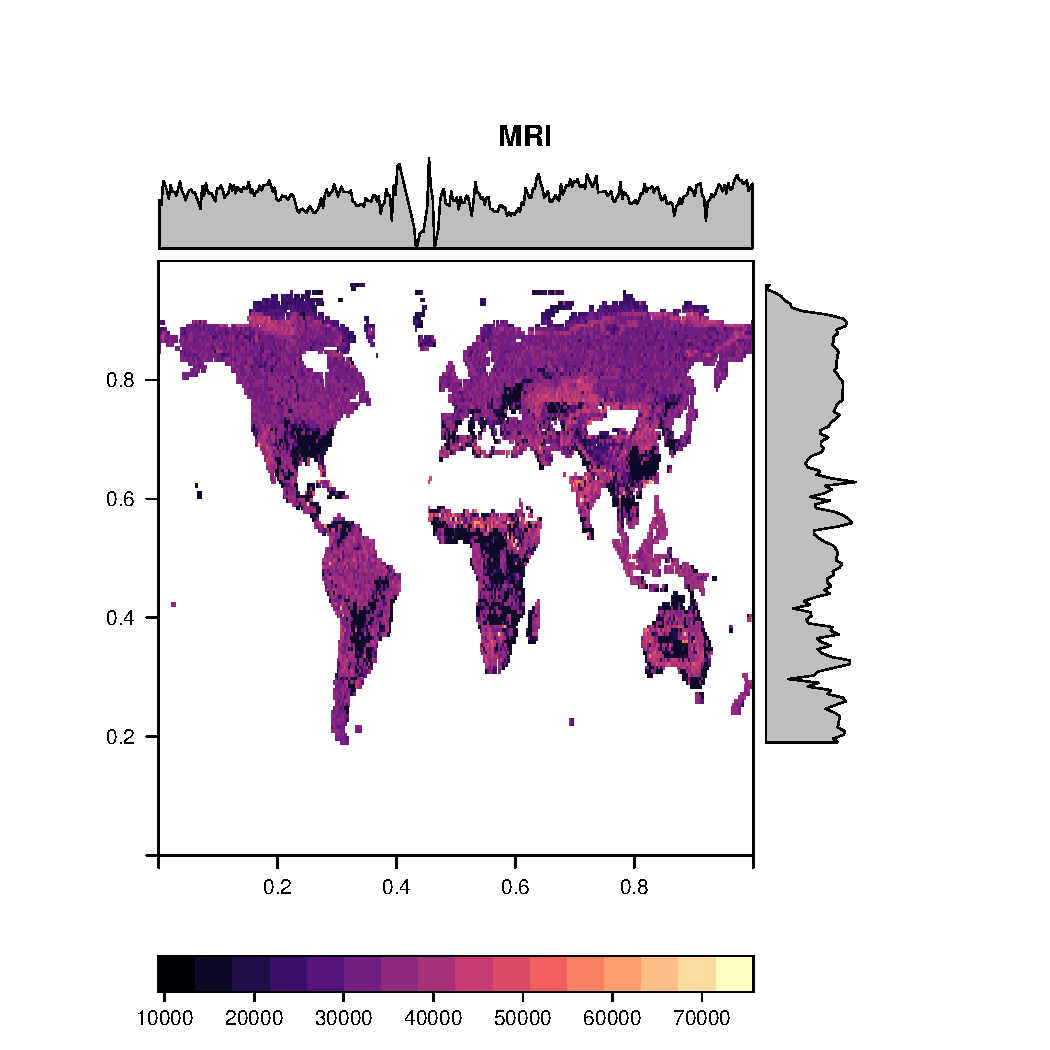
\includegraphics{Figures/corrP95MRI} % requires the graphicx package
   \caption{95\% quantile of the age distribution calculated for the reduced complexity version of the MRI model.}
\end{figure}

\begin{figure}[t]
   \centering
   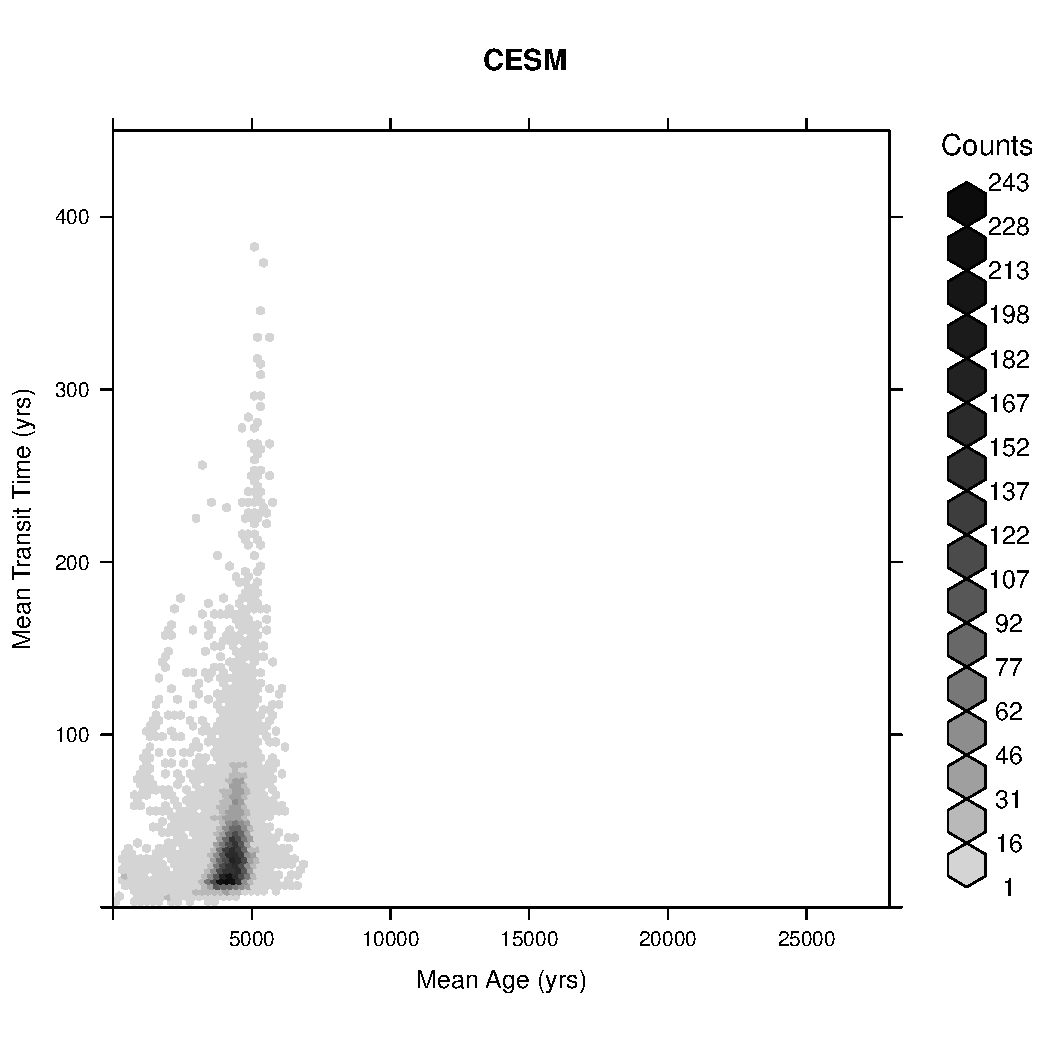
\includegraphics{Figures/hexbinplot_TTvsA_CESM} % requires the graphicx package
   \caption{Hexbin plot showing the relation between mean age and mean transit time for the CESM model. Darker colors are indicative of a larger number of grid cells with similar values.}
\end{figure}

\begin{figure}[t]
   \centering
   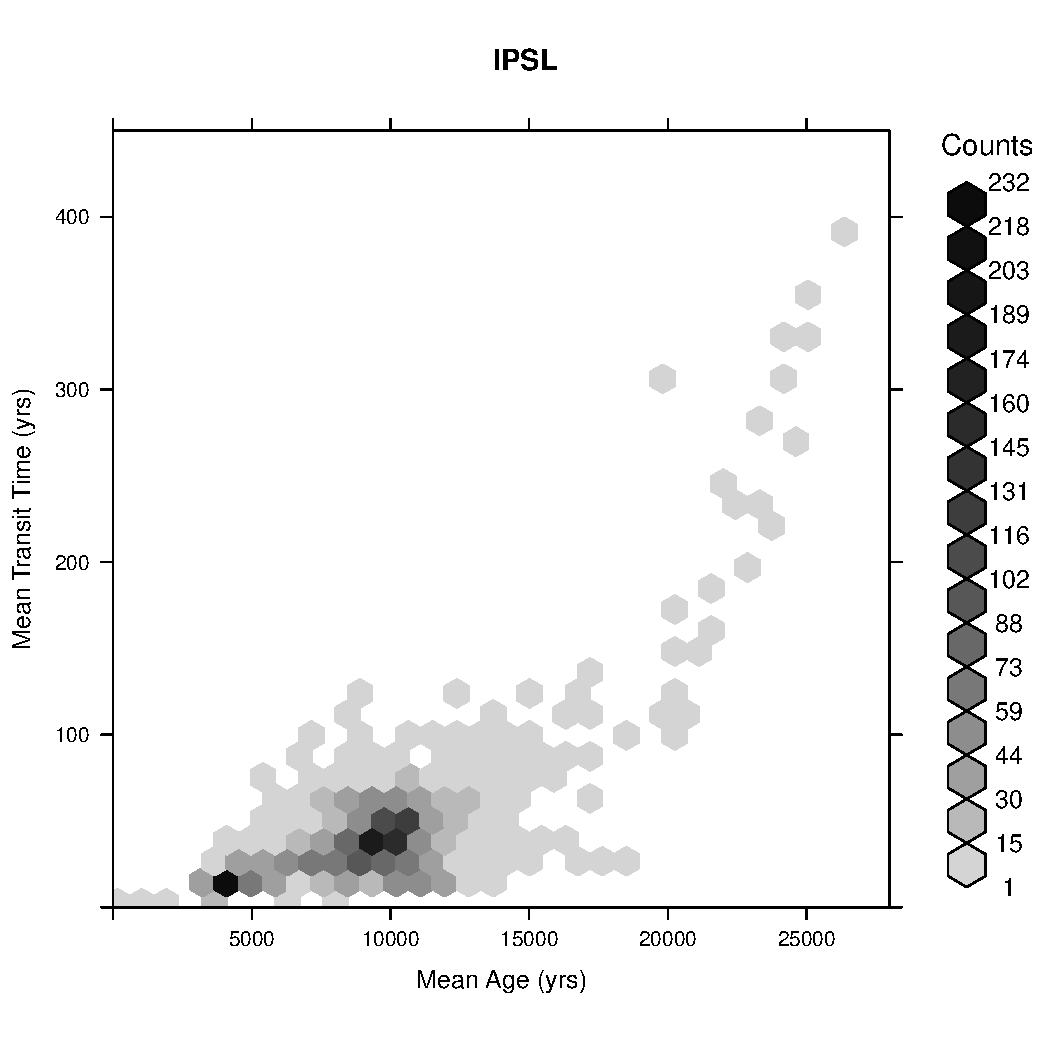
\includegraphics{Figures/hexbinplot_TTvsA_IPSL} % requires the graphicx package
   \caption{Hexbin plot showing the relation between mean age and mean transit time for the IPSL model. Darker colors are indicative of a larger number of grid cells with similar values.}
\end{figure}

\begin{figure}[t]
   \centering
   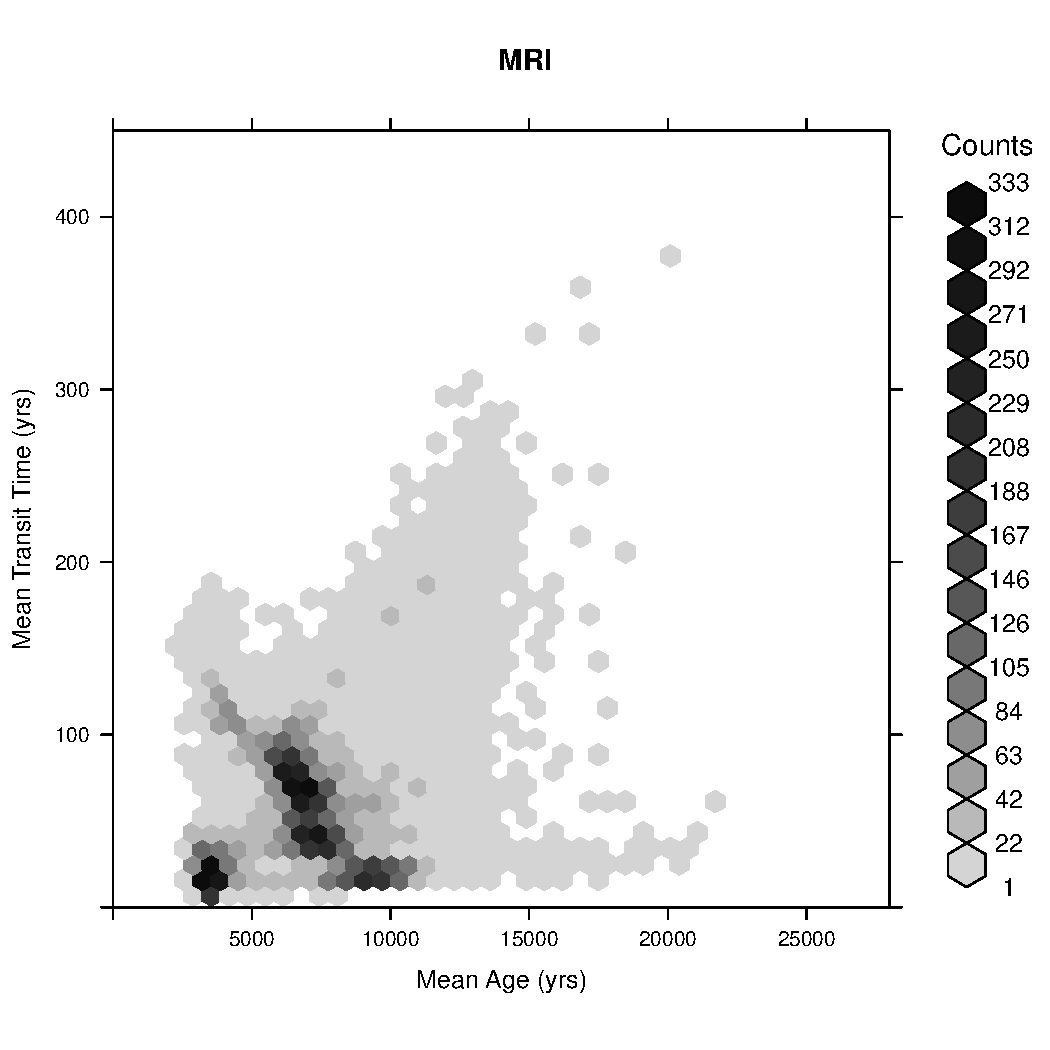
\includegraphics{Figures/hexbinplot_TTvsA_MRI} % requires the graphicx package
   \caption{Hexbin plot showing the relation between mean age and mean transit time for the MRI model. Darker colors are indicative of a larger number of grid cells with similar values.}
\end{figure}

\begin{figure}[t]
   \centering
   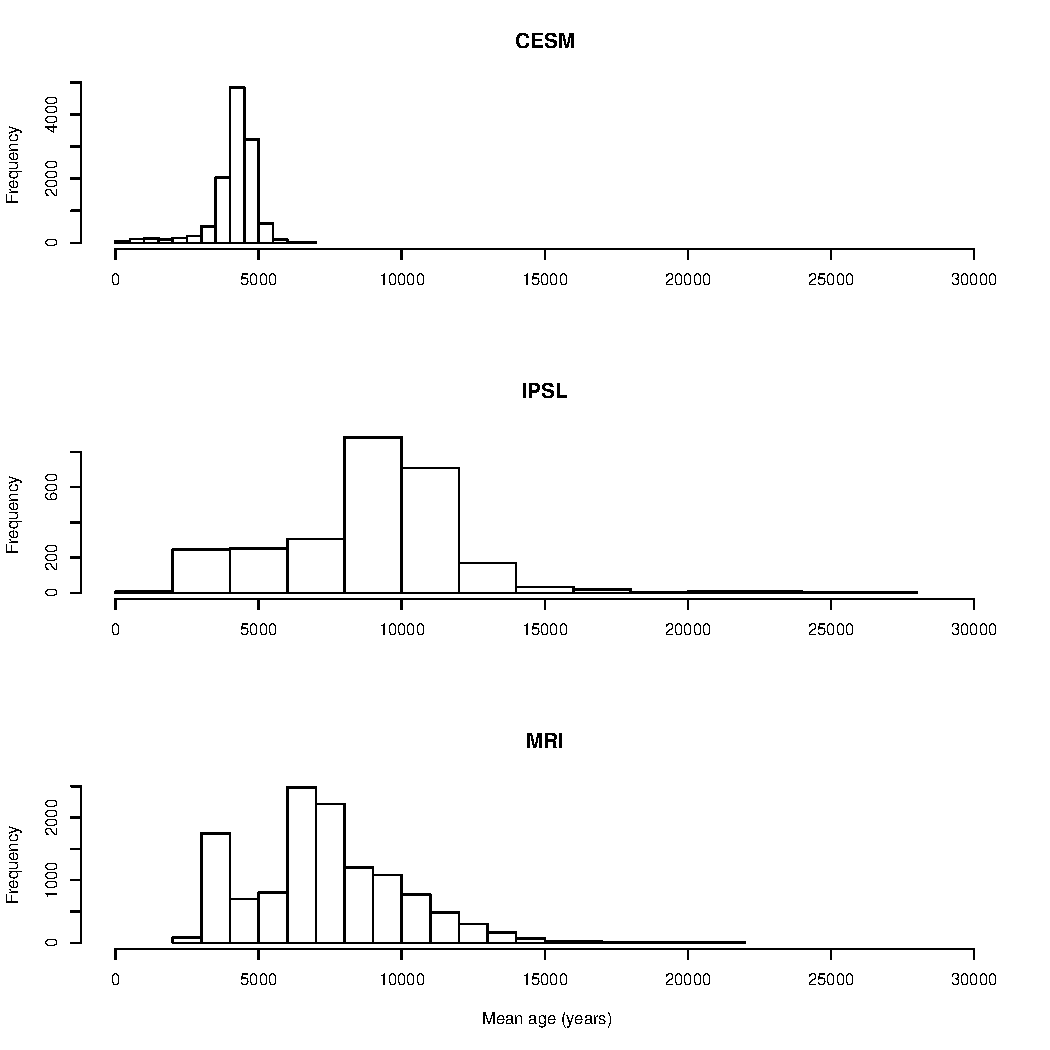
\includegraphics{Figures/corrSAESMs} % requires the graphicx package
   \caption{Histogram of mean ages for all models}
\end{figure}

\begin{figure}[t]
   \centering
   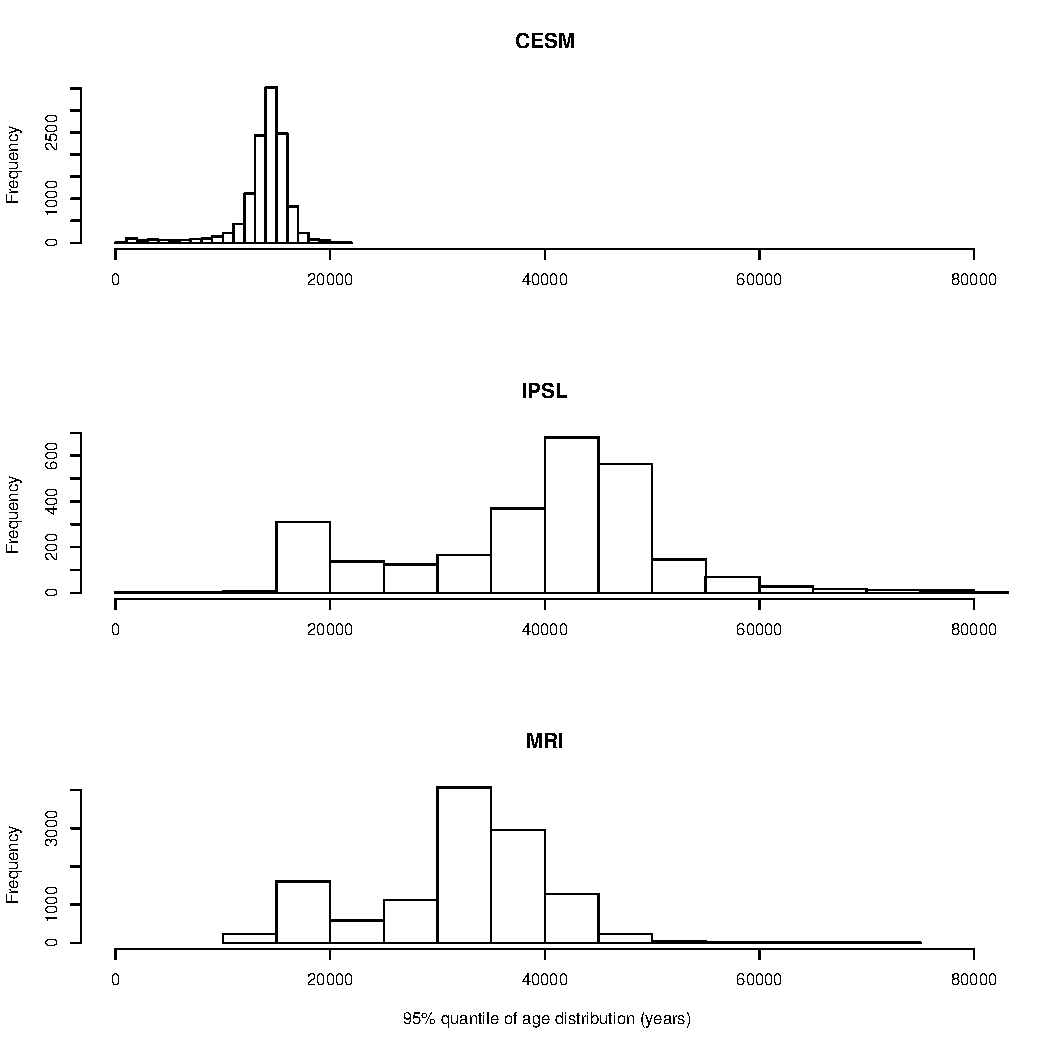
\includegraphics{Figures/corrP95ESMs} % requires the graphicx package
   \caption{Histogram of 95\% quantiles of the age distribution for all models}
\end{figure}


\end{document}  